\begin{multicols}{2}
\topic{Virtual Memory}
\subtopic{How is actual memory reached?}
\begin{itemize}[noitemsep, parsep=0.5em]
   \item Virtual addresses (VA) are translated to physical addresses (PA) to access actual memory.
   \item CPU works with VA but memory hardware uses PA.
   \item OS allocates memory and tracks process locations.
   \item Memory Management Unit (MMU) performs translation using info provided by the OS.
\end{itemize}

\begin{figure}[H]
   \centering
   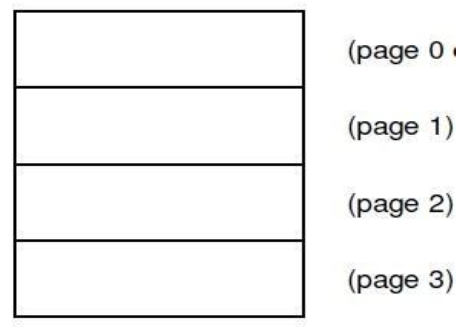
\includegraphics[width=0.45\linewidth]{figures/Paging1.png}
   \hspace{1em}
   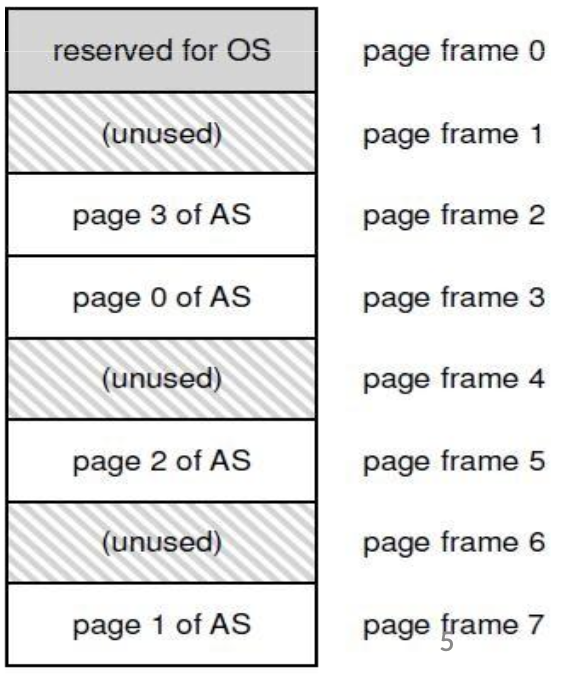
\includegraphics[width=0.45\linewidth]{figures/Paging2.png}
\end{figure}
% \begin{figure}[H]
%    \centering
%    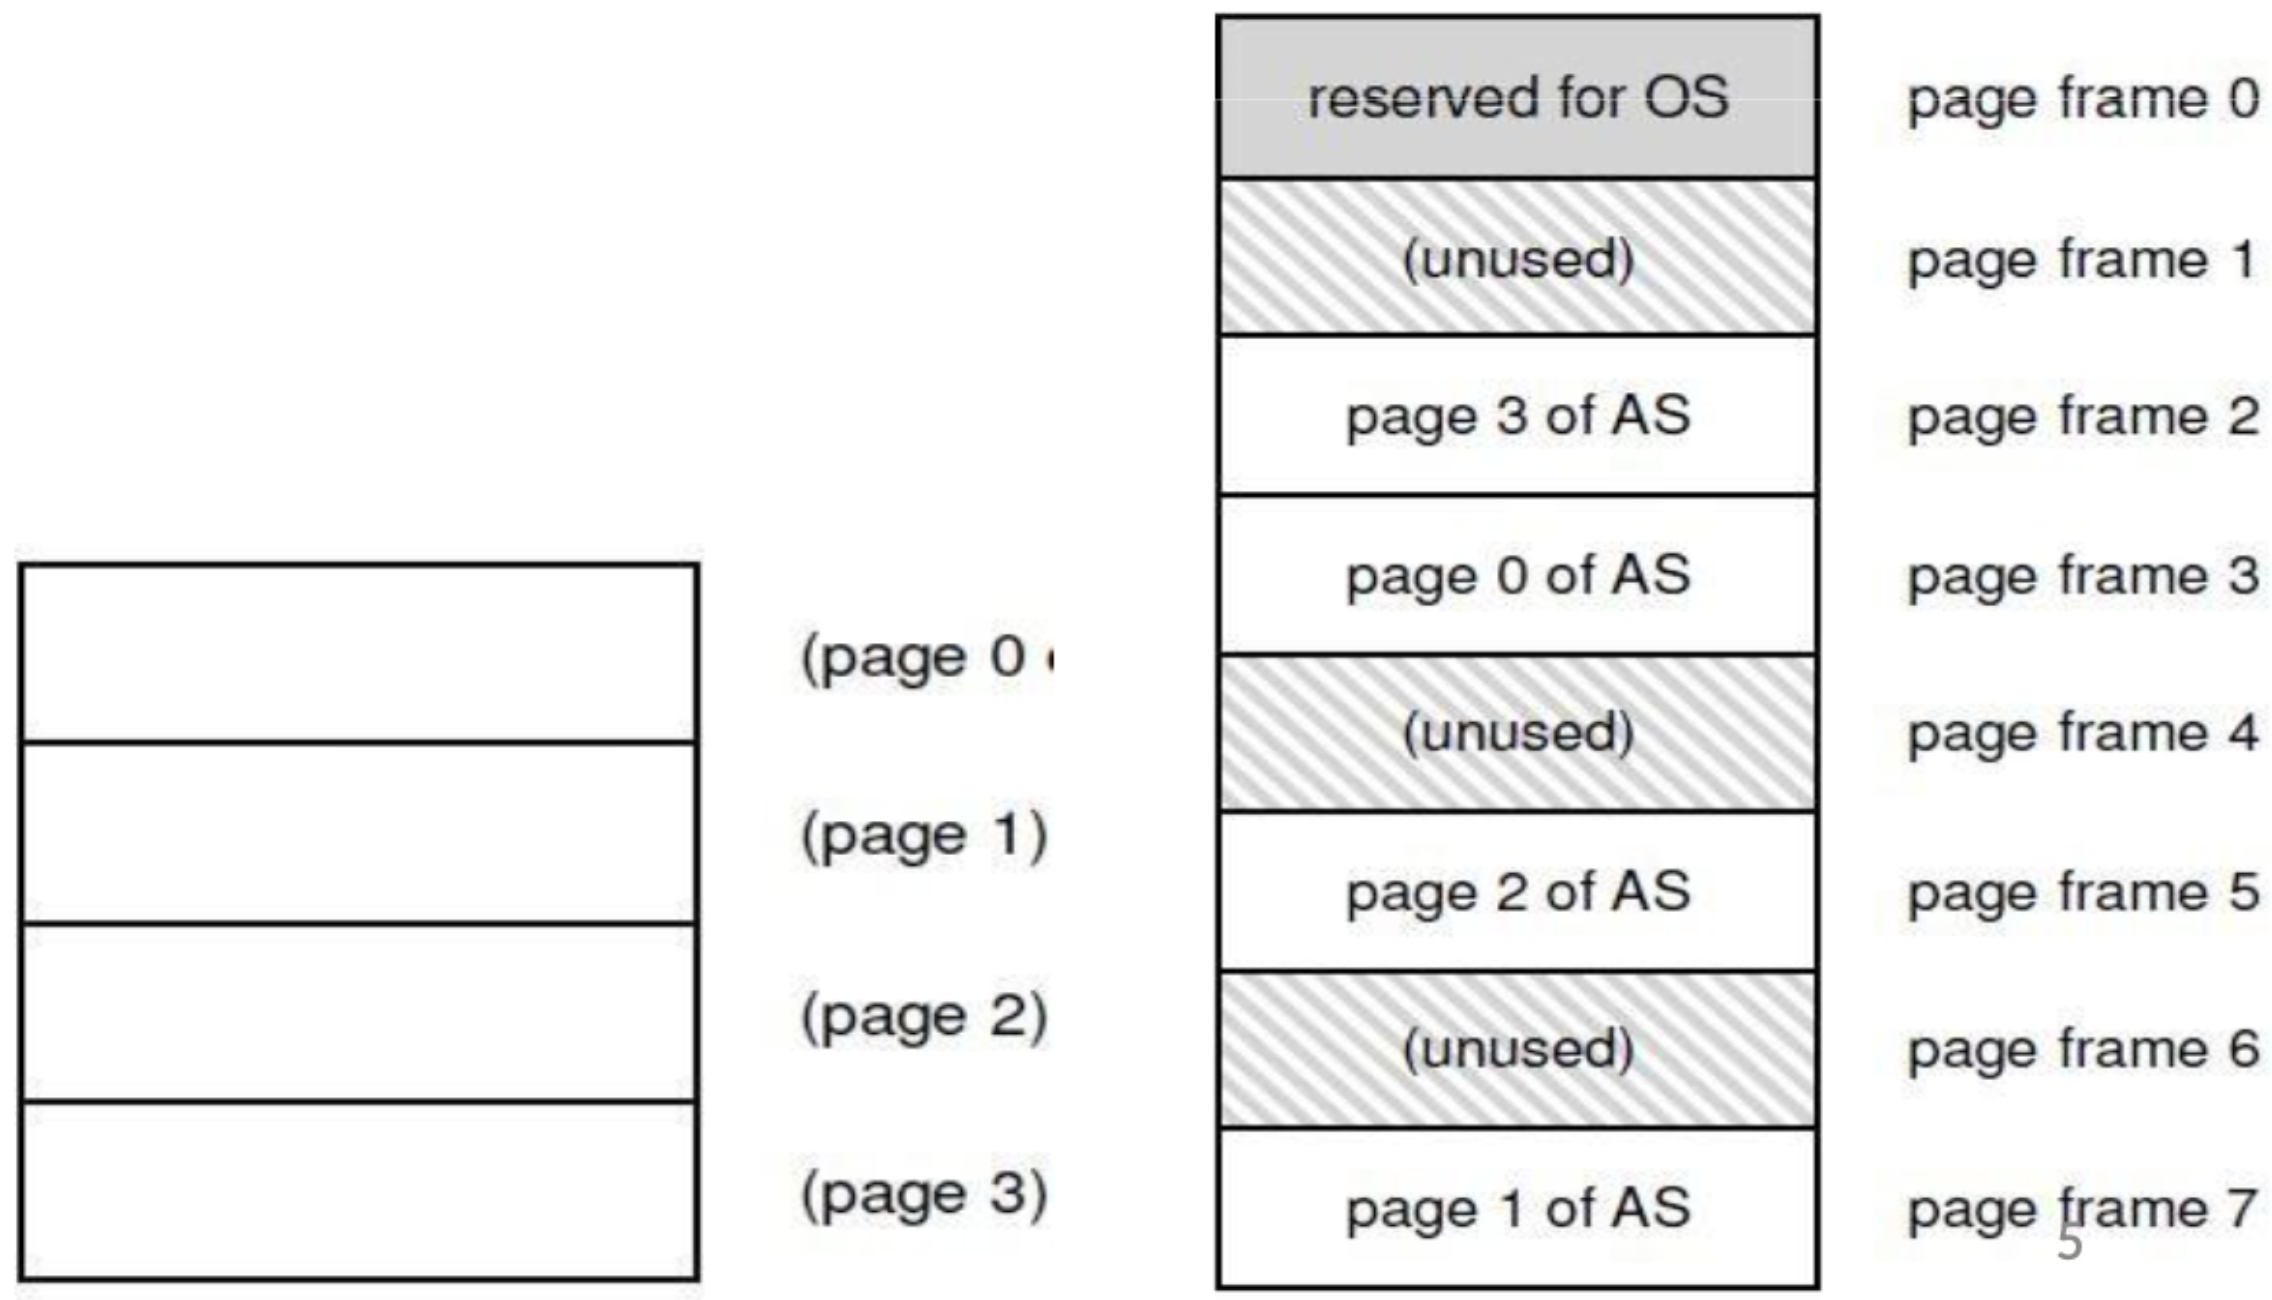
\includegraphics[width=0.45\linewidth]{figures/Paging.png}
% \end{figure}

\textbf{Example: Paging}
\begin{itemize}[noitemsep, parsep=0.5em]
   \item OS divides VA space into fixed size into \textbf{pages} and physical memory into \textbf{frames}.
   \item To allocate memory, a page is mapped to a free frame
   \item Page table stores mappings: virtual page $\to$ physical frame for a process.
   \item MMU uses page table to translate VA $\to$ PA.
\end{itemize}

\textbf{How does the OS allocate memory?}
\begin{itemize}[noitemsep, parsep=0.25em]
   \item OS needs memory for its data structures.
   \item For large allocations, OS allocates a page.
   \item For smaller allocations, OS uses various memory allocation algorithms.
   \begin{itemize}[noitemsep, parsep=0.5em]
      \item Cannot use libc and malloc in kernel!
   \end{itemize}
\end{itemize}

\vspace{1em}
\textbf{What are the system calls used for memory allocation?}
\begin{itemize}[noitemsep, parsep=0.5em]
    \item \texttt{malloc} is implemented by the C standard library.
    \item Uses algorithms for efficient memory allocation and free space management.
    \item To grow the heap, the C library typically uses the \texttt{brk}/\texttt{sbrk} system calls.
    \item Programs can also allocate page-sized memory regions with the \texttt{mmap()} system call.
    \item \texttt{mmap()} can request "anonymous" pages directly from the OS.
\end{itemize}

\begin{figure}[H]
   \centering
   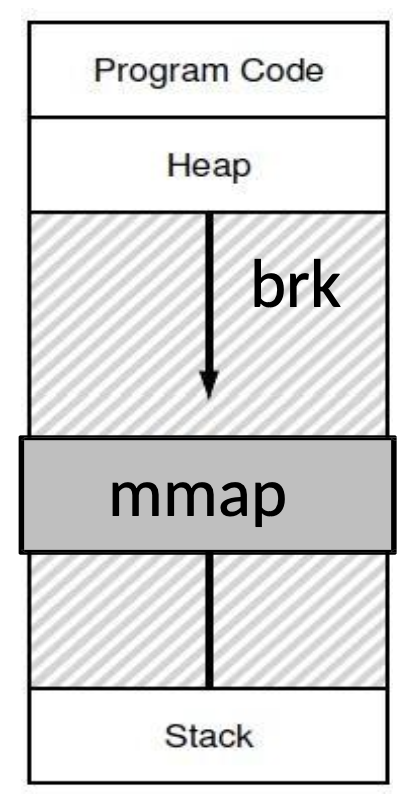
\includegraphics[width=3cm]{figures/syscall_memoery.png}
\end{figure}

\vspace{1em}
\textbf{What is the address space of the OS?}
\begin{itemize}[noitemsep, parsep=0.5em]
    \item The OS is not a separate process with its own address space.
    \item Instead, OS code is part of the address space of every process.
    \item A process sees the OS as part of its code (similar to a library).
    \item Page tables map the OS addresses to OS code.
\end{itemize}

\begin{figure}[H]
   \centering
   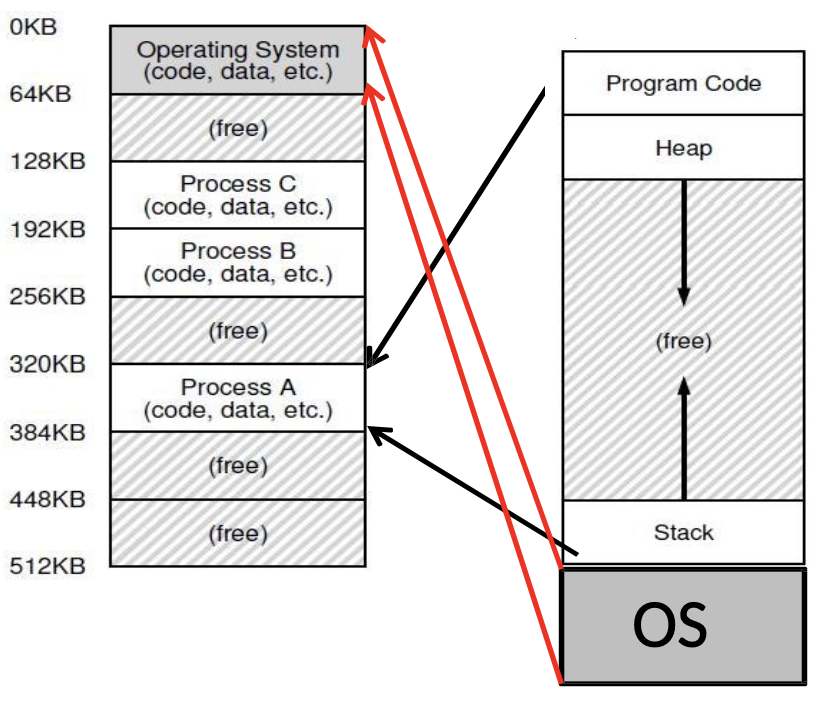
\includegraphics[width=0.8\linewidth]{figures/AddressSpace.png}
\end{figure}


\end{multicols}
